% Options for packages loaded elsewhere
\PassOptionsToPackage{unicode}{hyperref}
\PassOptionsToPackage{hyphens}{url}
%
\documentclass[
]{article}
\usepackage{amsmath,amssymb}
\usepackage{lmodern}
\usepackage{iftex}
\ifPDFTeX
  \usepackage[T1]{fontenc}
  \usepackage[utf8]{inputenc}
  \usepackage{textcomp} % provide euro and other symbols
\else % if luatex or xetex
  \usepackage{unicode-math}
  \defaultfontfeatures{Scale=MatchLowercase}
  \defaultfontfeatures[\rmfamily]{Ligatures=TeX,Scale=1}
\fi
% Use upquote if available, for straight quotes in verbatim environments
\IfFileExists{upquote.sty}{\usepackage{upquote}}{}
\IfFileExists{microtype.sty}{% use microtype if available
  \usepackage[]{microtype}
  \UseMicrotypeSet[protrusion]{basicmath} % disable protrusion for tt fonts
}{}
\makeatletter
\@ifundefined{KOMAClassName}{% if non-KOMA class
  \IfFileExists{parskip.sty}{%
    \usepackage{parskip}
  }{% else
    \setlength{\parindent}{0pt}
    \setlength{\parskip}{6pt plus 2pt minus 1pt}}
}{% if KOMA class
  \KOMAoptions{parskip=half}}
\makeatother
\usepackage{xcolor}
\usepackage[margin=1in]{geometry}
\usepackage{color}
\usepackage{fancyvrb}
\newcommand{\VerbBar}{|}
\newcommand{\VERB}{\Verb[commandchars=\\\{\}]}
\DefineVerbatimEnvironment{Highlighting}{Verbatim}{commandchars=\\\{\}}
% Add ',fontsize=\small' for more characters per line
\usepackage{framed}
\definecolor{shadecolor}{RGB}{248,248,248}
\newenvironment{Shaded}{\begin{snugshade}}{\end{snugshade}}
\newcommand{\AlertTok}[1]{\textcolor[rgb]{0.94,0.16,0.16}{#1}}
\newcommand{\AnnotationTok}[1]{\textcolor[rgb]{0.56,0.35,0.01}{\textbf{\textit{#1}}}}
\newcommand{\AttributeTok}[1]{\textcolor[rgb]{0.77,0.63,0.00}{#1}}
\newcommand{\BaseNTok}[1]{\textcolor[rgb]{0.00,0.00,0.81}{#1}}
\newcommand{\BuiltInTok}[1]{#1}
\newcommand{\CharTok}[1]{\textcolor[rgb]{0.31,0.60,0.02}{#1}}
\newcommand{\CommentTok}[1]{\textcolor[rgb]{0.56,0.35,0.01}{\textit{#1}}}
\newcommand{\CommentVarTok}[1]{\textcolor[rgb]{0.56,0.35,0.01}{\textbf{\textit{#1}}}}
\newcommand{\ConstantTok}[1]{\textcolor[rgb]{0.00,0.00,0.00}{#1}}
\newcommand{\ControlFlowTok}[1]{\textcolor[rgb]{0.13,0.29,0.53}{\textbf{#1}}}
\newcommand{\DataTypeTok}[1]{\textcolor[rgb]{0.13,0.29,0.53}{#1}}
\newcommand{\DecValTok}[1]{\textcolor[rgb]{0.00,0.00,0.81}{#1}}
\newcommand{\DocumentationTok}[1]{\textcolor[rgb]{0.56,0.35,0.01}{\textbf{\textit{#1}}}}
\newcommand{\ErrorTok}[1]{\textcolor[rgb]{0.64,0.00,0.00}{\textbf{#1}}}
\newcommand{\ExtensionTok}[1]{#1}
\newcommand{\FloatTok}[1]{\textcolor[rgb]{0.00,0.00,0.81}{#1}}
\newcommand{\FunctionTok}[1]{\textcolor[rgb]{0.00,0.00,0.00}{#1}}
\newcommand{\ImportTok}[1]{#1}
\newcommand{\InformationTok}[1]{\textcolor[rgb]{0.56,0.35,0.01}{\textbf{\textit{#1}}}}
\newcommand{\KeywordTok}[1]{\textcolor[rgb]{0.13,0.29,0.53}{\textbf{#1}}}
\newcommand{\NormalTok}[1]{#1}
\newcommand{\OperatorTok}[1]{\textcolor[rgb]{0.81,0.36,0.00}{\textbf{#1}}}
\newcommand{\OtherTok}[1]{\textcolor[rgb]{0.56,0.35,0.01}{#1}}
\newcommand{\PreprocessorTok}[1]{\textcolor[rgb]{0.56,0.35,0.01}{\textit{#1}}}
\newcommand{\RegionMarkerTok}[1]{#1}
\newcommand{\SpecialCharTok}[1]{\textcolor[rgb]{0.00,0.00,0.00}{#1}}
\newcommand{\SpecialStringTok}[1]{\textcolor[rgb]{0.31,0.60,0.02}{#1}}
\newcommand{\StringTok}[1]{\textcolor[rgb]{0.31,0.60,0.02}{#1}}
\newcommand{\VariableTok}[1]{\textcolor[rgb]{0.00,0.00,0.00}{#1}}
\newcommand{\VerbatimStringTok}[1]{\textcolor[rgb]{0.31,0.60,0.02}{#1}}
\newcommand{\WarningTok}[1]{\textcolor[rgb]{0.56,0.35,0.01}{\textbf{\textit{#1}}}}
\usepackage{longtable,booktabs,array}
\usepackage{calc} % for calculating minipage widths
% Correct order of tables after \paragraph or \subparagraph
\usepackage{etoolbox}
\makeatletter
\patchcmd\longtable{\par}{\if@noskipsec\mbox{}\fi\par}{}{}
\makeatother
% Allow footnotes in longtable head/foot
\IfFileExists{footnotehyper.sty}{\usepackage{footnotehyper}}{\usepackage{footnote}}
\makesavenoteenv{longtable}
\usepackage{graphicx}
\makeatletter
\def\maxwidth{\ifdim\Gin@nat@width>\linewidth\linewidth\else\Gin@nat@width\fi}
\def\maxheight{\ifdim\Gin@nat@height>\textheight\textheight\else\Gin@nat@height\fi}
\makeatother
% Scale images if necessary, so that they will not overflow the page
% margins by default, and it is still possible to overwrite the defaults
% using explicit options in \includegraphics[width, height, ...]{}
\setkeys{Gin}{width=\maxwidth,height=\maxheight,keepaspectratio}
% Set default figure placement to htbp
\makeatletter
\def\fps@figure{htbp}
\makeatother
\setlength{\emergencystretch}{3em} % prevent overfull lines
\providecommand{\tightlist}{%
  \setlength{\itemsep}{0pt}\setlength{\parskip}{0pt}}
\setcounter{secnumdepth}{-\maxdimen} % remove section numbering
\ifLuaTeX
  \usepackage{selnolig}  % disable illegal ligatures
\fi
\IfFileExists{bookmark.sty}{\usepackage{bookmark}}{\usepackage{hyperref}}
\IfFileExists{xurl.sty}{\usepackage{xurl}}{} % add URL line breaks if available
\urlstyle{same} % disable monospaced font for URLs
\hypersetup{
  pdftitle={Quarta\_Assignment},
  pdfauthor={Ankit},
  hidelinks,
  pdfcreator={LaTeX via pandoc}}

\title{Quarta\_Assignment}
\author{Ankit}
\date{2023-04-27}

\begin{document}
\maketitle

\hypertarget{how-i-met-your-mother}{%
\section{How I met your Mother}\label{how-i-met-your-mother}}

How I Met Your Mother (often abbreviated as HIMYM) is an American
sitcom, created by Craig Thomas and Carter Bays for CBS. The series,
which aired from September 19, 2005 to March 31, 2014, follows the main
character, Ted Mosby, and his group of friends in New York City's
Manhattan. As a framing device, Ted, in 2030, recounts to his son, Luke,
and daughter, Penny, the events from September 2005 to May 2013 that led
him to meet their mother. How I Met Your Mother, is a joint production
by Bays \& Thomas Productions and 20th Century Fox Television and
syndicated by 20th Television (now Disney-ABC Domestic Television).

\hypertarget{seasons-information}{%
\section{Seasons information}\label{seasons-information}}

\begin{longtable}[]{@{}llll@{}}
\toprule()
Season & Episodes & Originally aired & Rank \\
\midrule()
\endhead
1 & 22 & September 19, 2005 & May 15, 2006 \\
2 & 22 & September 18, 2006 & May 14, 2007 \\
3 & 20 & September 24, 2007 & May 19, 2008 \\
4 & 24 & September 22, 2008 & May 18, 2009 \\
5 & 24 & September 21, 2009 & May 24, 2010 \\
6 & 24 & September 20, 2010 & May 16, 2011 \\
7 & 24 & September 19, 2011 & May 14, 2012 \\
8 & 24 & September 24, 2012 & May 13, 2013 \\
9 & 24 & September 23, 2013 & March 31, 2014 \\
\bottomrule()
\end{longtable}

\hypertarget{how-i-met-you-mother-poster}{%
\subsection{How I Met you Mother
poster}\label{how-i-met-you-mother-poster}}

\begin{Shaded}
\begin{Highlighting}[]
\FunctionTok{library}\NormalTok{(ggplot2)}
\end{Highlighting}
\end{Shaded}

\begin{verbatim}
## Warning: package 'ggplot2' was built under R version 4.2.2
\end{verbatim}

\begin{Shaded}
\begin{Highlighting}[]
\CommentTok{\# create a data frame with the season and viewers data}
\NormalTok{season\_viewers }\OtherTok{\textless{}{-}} \FunctionTok{data.frame}\NormalTok{(}
  \AttributeTok{season =} \FunctionTok{c}\NormalTok{(}\DecValTok{1}\NormalTok{, }\DecValTok{2}\NormalTok{, }\DecValTok{3}\NormalTok{, }\DecValTok{4}\NormalTok{, }\DecValTok{5}\NormalTok{, }\DecValTok{6}\NormalTok{, }\DecValTok{7}\NormalTok{, }\DecValTok{8}\NormalTok{, }\DecValTok{9}\NormalTok{),}
  \AttributeTok{viewers =} \FunctionTok{c}\NormalTok{(}\FloatTok{9.47}\NormalTok{, }\FloatTok{8.94}\NormalTok{, }\FloatTok{8.21}\NormalTok{, }\FloatTok{9.42}\NormalTok{, }\FloatTok{8.60}\NormalTok{, }\FloatTok{8.79}\NormalTok{, }\FloatTok{9.67}\NormalTok{, }\FloatTok{9.02}\NormalTok{, }\FloatTok{10.51}\NormalTok{)}
\NormalTok{)}

\CommentTok{\# create a line graph with season on the x{-}axis and viewers on the y{-}axis}
\FunctionTok{ggplot}\NormalTok{(season\_viewers, }\FunctionTok{aes}\NormalTok{(}\AttributeTok{x =}\NormalTok{ season, }\AttributeTok{y =}\NormalTok{ viewers)) }\SpecialCharTok{+}
  \FunctionTok{geom\_line}\NormalTok{() }\SpecialCharTok{+}
  \FunctionTok{geom\_point}\NormalTok{() }\SpecialCharTok{+}
  \FunctionTok{xlab}\NormalTok{(}\StringTok{"Season"}\NormalTok{) }\SpecialCharTok{+}
  \FunctionTok{ylab}\NormalTok{(}\StringTok{"Viewers (millions)"}\NormalTok{) }\SpecialCharTok{+}
  \FunctionTok{ggtitle}\NormalTok{(}\StringTok{"Viewership by Season"}\NormalTok{)}
\end{Highlighting}
\end{Shaded}

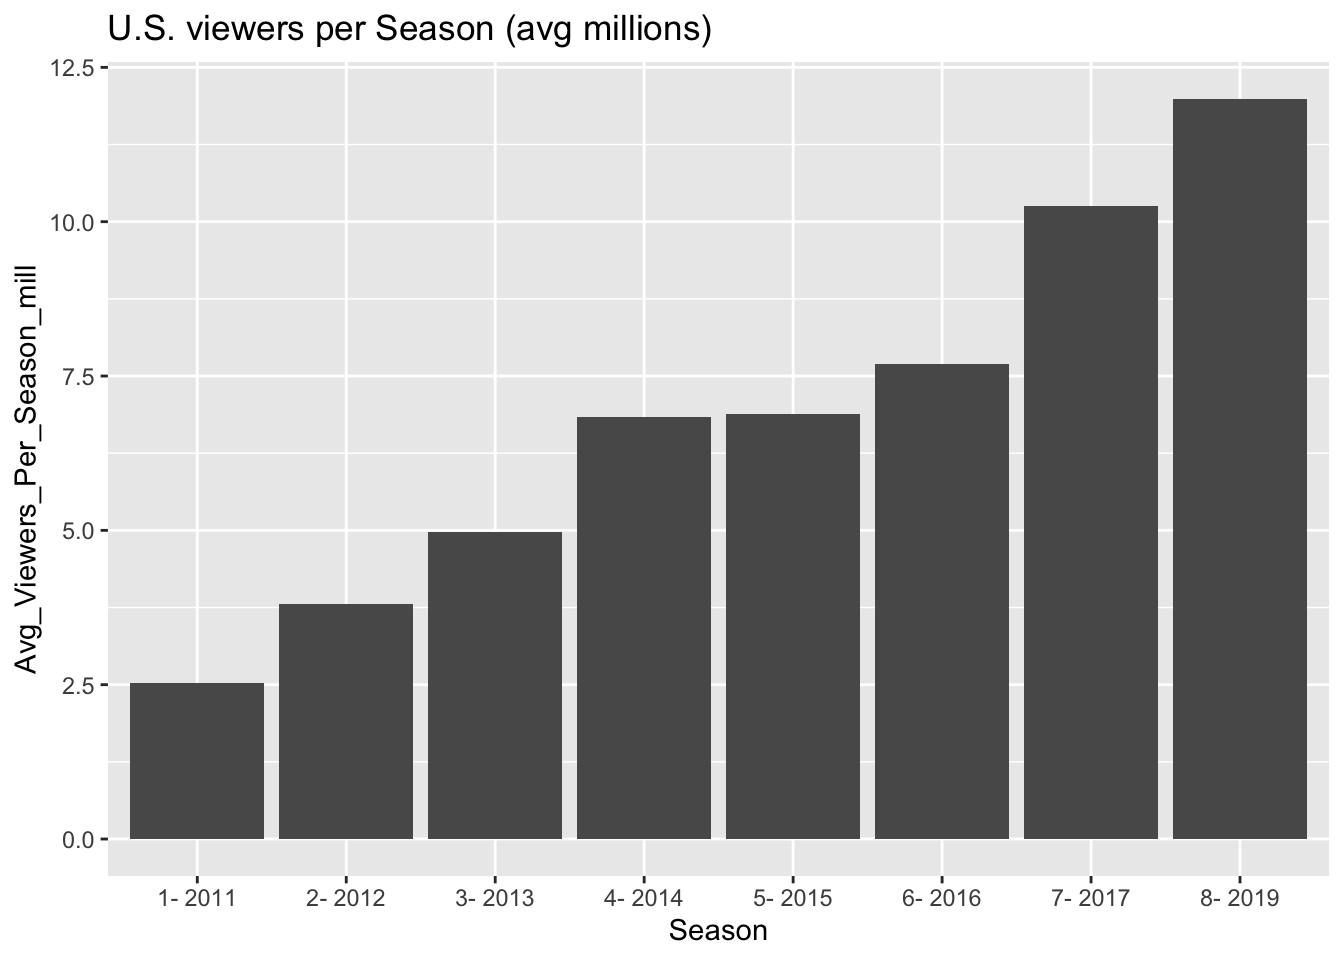
\includegraphics{Quarto_Assignment_1_files/figure-latex/unnamed-chunk-1-1.pdf}

The data shows that there have been significant changes in viewership
throughout the nine seasons of the TV show. For example, the viewership
decreased by an average of 0.27 million between seasons 1 and 2, and
then increased by an average of 0.27 million between seasons 2 and 3.
However, the viewership then decreased again by an average of 0.13
million between seasons 3 and 4, and this trend continued until season
6, where the viewership hit its lowest point at an average of 7.15
million viewers. After that, the viewership started to pick up again,
with season 9 having the highest average viewership of 10.51 million.
Overall, the viewership changes were significant and showed a clear
trend of ups and downs throughout the show's run.

\end{document}
